\documentclass[letter]{article}
\usepackage[english]{babel}
\selectlanguage{english}
\usepackage[utf8]{inputenc}
\usepackage[T1]{fontenc}
\usepackage{color}
\usepackage{biblatex}
\usepackage[autostyle]{csquotes}
\addbibresource{sample.bib}

\usepackage[a4paper,top=3cm,bottom=2cm,left=3cm,right=3cm,marginparwidth=1.75cm]{geometry}

\usepackage{amsmath, amsthm, amsfonts}
\usepackage{graphicx}
\usepackage[colorinlistoftodos]{todonotes}
\usepackage[colorlinks=true, allcolors=blue]{hyperref}

\title{The Schrodinger Equation and Other Cool Physics Concepts Explained}
\author{Nicolás Díaz Durana}
\date{February 27, 2021}

\begin{document}
\maketitle

%%%%%%%%%%%%%%%%%%%%%%%%%%%%%%%%%%%%%%%%%%%%%%%%%%%%%%%%%%
%%%%%%%%%%%%%%%%%%%%%%%%%%%%%%%%%%%%%%%%%%%%%%%%%%%%%%%%%%

\begin{enumerate}
    
    \item \textbf{Deducing the Schrödinger equation.}\\
    $$\frac{-\hbar^2}{2m}\frac{\partial^2\psi(x,t)}{\partial x^2}+V(x,t)\psi(x,t)=i\hbar \frac{\partial \psi(x,t)}{\partial t}$$\\
    \paragraph{}One possible path to understanding the origins of the Schrödinger equation is to start with a classical equation that links the total energy to the sum of kinetic and potential energy. 
    \paragraph{}In order to adapt this principle to quantum wave functions, consider the equation
    \begin{equation}
        \begin{split}
            E &= hf =\hbar \omega\\
        \end{split}
    \end{equation}
    \paragraph{}where $E$ is the energy of the photon, $f$ is its frequency, $\omega$ is the angular frequency and $\hbar$ stands for the modified Planck constant, defined as $\hbar=\frac{h}{2\pi}$. This equation was developed by Max Planck and Albert Einstein at the beginning of the 1900's. 
    \paragraph{} Around the same time, Louis de Broglie stood for the idea that particles behave like waves in the quantum world. Their momentum can be summarized as 
    \begin{equation}
        \begin{split}
            p &= \frac{E}{c}=\frac{\hbar \omega}{c}\\
        \end{split}
    \end{equation}
    \paragraph{} Here we see equation 1 combined with the expression $\frac{E}{c}=p$, which comes from James Maxwell's research on radiation pressure. It relates momentum ($p$), energy ($E$) and the speed of light ($c$). This new equation can be taken one step forward:
    \begin{equation}
        \begin{split}
            p   &= \frac{\hbar \omega}{c}\\
                &= \frac{\hbar(2\pi f)}{c}\\
                &= \frac{\hbar(2\pi \frac{c}{\lambda})}{c}\\
                &= \frac{\hbar 2\pi}{\lambda}\\
        \end{split}
    \end{equation}
    \paragraph{} Equation 3 shows the existing relation between the frequency ($f$) of a wave and its wavelength ($\lambda$) and speed ($c$): $f=\frac{c}{\lambda}$. When combined with the momentum equation (Eq. 2), we arrive to the de Broglie relation, which articulates the behavior of particles and waves into the concept of \textit{wave-particle duality}:
    \begin{equation}
        \begin{split}
            p &= \hbar k\\
        \end{split}
    \end{equation}
    \paragraph{} The definition of wavenumber allows us to replace $\frac{2\pi}{\lambda}$ with $k$. On the other hand, the classical equation for kinetic energy is
    \begin{equation}
        \begin{split}
            KE  &= \frac{1}{2}mv^2\\
        \end{split}
    \end{equation}
    \paragraph{} Since the momentum can be expressed as the product of mass and velocity ($p=mv$) and we defined momentum as $p=\hbar k$ in equation 4, we can rewrite as follows:
    \begin{equation}
        \begin{split}
            KE  &= \frac{p^2}{2m}\\
                &= \frac{\hbar^2 k^2}{2m}\\
        \end{split}
    \end{equation}
    \paragraph{} The total energy ($E$) is expressed as the sum of the kinetic energy and the potential energy. Also, in equation 1 we defined $E=\hbar \omega$. With this in mind, we get
    \begin{equation}
        \begin{split}
            E   &= KE+V\\
            E   &=\frac{\hbar^2 k^2}{2m}+V\\
            E   &= \hbar \omega = \frac{\hbar^2 k^2}{2m}+V\\
        \end{split}
    \end{equation}
    \paragraph{} By applying this equation to the quantum wave function, we will be able to deduce the Schrödinger equation. To this end, lets assume that the quantum wavefuction has the form of a wave for which the surfaces of constant phase are flat planes. 
    \begin{equation}
        \begin{split}
            \psi(x,t) &= Ae^{i(kx-\omega t)}
        \end{split}
    \end{equation}
    \paragraph{}Equation 8 is a wavefunction in which a plane wave propagates in the positive x-direction. The wave amplitude is represented by $A$, $\omega$ stands for the angular frequency of the wave and $k$ is the wave number.
    \paragraph{} The following steps will allow us to write $\omega$ and $k$ in terms of the wavefunction $\psi$ and its derivatives, which will eventually lead us to the most common form of the Schrödinger equation. 
    \paragraph{}We will start by taking the first partial derivative of $\psi(x,t)$ with respect to time:
    \begin{equation}
        \begin{split}
            \frac{\partial \psi(x,t)}{\partial t} 
            &= \frac{\partial [Ae^{i(kx-\omega t)}]}{\partial t}\\
            &= -i\omega[Ae^{i(kx-\omega t)}]\\
            &= -i\omega \psi(x,t)\\
        \end{split}
    \end{equation}
    \paragraph{} Since $\frac{\partial \psi}{\partial t}=-i\omega\psi$, we can express $\omega$ as
    \begin{equation}
        \begin{split}
            \omega 
            &= \frac{1}{-i\psi}\frac{\partial \psi}{\partial t}\\
            &= i\frac{1}{\psi}\frac{\partial \psi}{\partial t}\\
        \end{split}
    \end{equation}
    \paragraph{}The next step consists in taking the first partial derivative of $\psi(x,t)$ with respect to position:
    \begin{equation}
        \begin{split}
            \frac{\partial \psi(x,t)}{\partial x} 
            &= \frac{\partial [Ae^{i(kx-\omega t)}]}{\partial x}\\
            &= ik[Ae^{i(kx-\omega t)}]\\
            &= ik \psi(x,t)\\
        \end{split}
    \end{equation}
    \paragraph{}and then taking the second partial derivative of the plane-wave function, once again with respect to position:
    \begin{equation}
        \begin{split}
            \frac{\partial^2 \psi(x,t)}{\partial x^2} 
            &= \frac{\partial [ikAe^{i(kx-\omega t)}]}{\partial x}\\
            &= ik[ikAe^{i(kx-\omega t)}]\\
            &= -k^2 \psi(x,t)\\
        \end{split}
    \end{equation}
    \paragraph{}At this point, we have the following equations:
    \begin{equation}
        \begin{split}
            \frac{\partial\psi}{\partial t}
            &= -i\omega\psi\\
            \end{split}
    \end{equation}
    \begin{equation}
        \begin{split}
            \frac{\partial^2 \psi}{\partial x^2}
            &= -k^2\psi\\
        \end{split}
    \end{equation}
    \paragraph{}which can respectively be rewritten as
    \begin{equation}
        \begin{split}
            \omega 
            &= i\frac{1}{\psi}\frac{\partial \psi}{\partial t}\\
        \end{split}
    \end{equation}
    \begin{equation}
        \begin{split}
            k^2
            &= -\frac{1}{\psi}\frac{\partial^2 \psi}{\partial x^2}
        \end{split}
    \end{equation}
     \paragraph{}Substituting the expression for $\omega$ from Eq. 15 into the left side of Eq. 7, we get
     \begin{equation}
         \begin{split}
             E  &= \hbar\omega\\
                &= \hbar\bigg(i\frac{1}{\psi}\frac{\partial\psi}{\partial t}\bigg)\\
                &= i\hbar\frac{1}{\psi}\frac{\partial\psi}{\partial t}
         \end{split}
     \end{equation}
    \paragraph{}Similarly, substituting the expression for $k^2$ from Eq. 16 into the right side of Eq. 7, we obtain
    \begin{equation}
        \begin{split}
            \frac{h^2k^2}{2m}+V &= \frac{h^2}{2m}\bigg(-\frac{1}{\psi}\frac{\partial^2\psi}{\partial x^2}\bigg)+V
        \end{split}
    \end{equation}
    \paragraph{}Combining both sides of equation 7 after these substitutions, we get the equation for total energy in the following terms:
    \begin{equation}
        \begin{split}
            i\hbar\frac{1}{\psi}\frac{\partial[\psi(x,t)]}{\partial t}
            &= -\frac{h^2}{2m}\frac{1}{\psi}\frac{\partial^2[\psi(x,t)]}{\partial x^2}+V
        \end{split}
    \end{equation}
    \paragraph{}Finally, if we modify the equation by multiplying it by the wavefunction $\psi(x,t)$, we reach the Schrödinger equation:
    \begin{equation}
        \begin{split}
            \frac{-\hbar^2}{2m}\frac{\partial^2\psi(x,t)}{\partial x^2}+V(x,t)\psi(x,t)
            &= i\hbar \frac{\partial \psi(x,t)}{\partial t}\\
        \end{split}
    \end{equation}
    \newpage
%%%%%%%%%%%%%%%%%%%%%%%%%%%%%%%%%%%%%%%%%%%%%%%%%%%%%%%%%%
    \item \textbf{Explaining what the Planck constant is and where it comes from.}
    \paragraph{} The Planck constant is a theoretical concept discovered and popularized by physicist Max Planck at the beginning of the twentieth century. 
    Planck was interested in explaining why black body radiation has a limited energy spectrum. In other words, he was interested in understanding the behavior of light and its wavelengths.
    \paragraph{}Light with a longer wavelength than red light is called "infra-red", whereas light with a shorter wavelength than blue light is called "ultra-violet". The shortest wavelength light is called "gamma radiation". An object with a certain temperature will emit light in the infra-red section of the spectrum. If the temperature of the object rises, the wavelength of the radiation will decrease. In general, the hotter an object, the shorter the wavelength of its light. 
    \paragraph{}In the final years of the nineteenth century, there was no precise formula to describe this behavior. This is what became known as the "black body problem".
    \paragraph{}In his works about the black body problem, Planck conjectured that energy is quantized. He assumed that the energy of the emitted light of an object was made up of a great number of "packets" of energy. These tiny pieces were fundamental constant units of energy in Nature, which Planck called "the quantum of action". This is what is known today as $\textit{\textbf{h}}$, the Planck's constant.
    \paragraph{}Steiner (2012) describes one of the earliest experiments which investigated the photoelectric effect that allows an intuitive approach to Planck's constant:
    \vspace{1mm}
    \begin{center}
        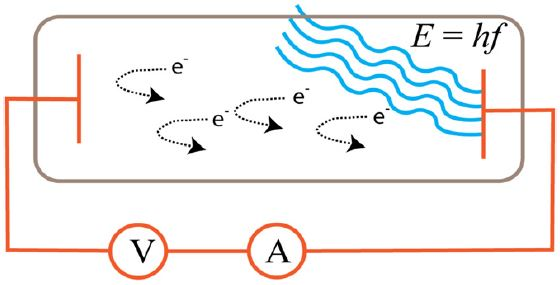
\includegraphics[width=.5\textwidth]{experiment.JPG}
    \end{center}
    \vspace{1mm}
    \blockquote{"Inside a vacuum chamber, light of different frequencies ejects electrons from a metal plate. The energy of the electrons is found by increasing the voltage, $V$, until there is no more measured current, $A$. The impinging electromagnetic light energy must exceed a work function, $W$, a characteristic of the metal. Graphing the current-stopping voltage against the impinging light’s frequency produces a line where the slope is the ratio $h/e$, where $e$ is the elementary charge."\cite{Steiner, R. (2012)}}
    \paragraph{}As it can be seen, the relation in terms of energy or work is $eV = hf-W$. An experiment of this sort constitutes one of the first ever indirect determinations of the constant $h$. However, it was not yet formally measured. In fact, physicists continue to research on new methods to measure accurately the Planck's constant.
    \paragraph{}The equation that describes the way the energy of light gets its values from is $E_{photon} = nhv$, where $n$ is a positive integer, $h$ is the Planck's constant and $v$ is the frequency of the light.
    \paragraph{} The modern value for Planck´s constant is $6.6260695729 \times10^{-34}$ kg m$^2/$s. 
    \newpage

%%%%%%%%%%%%%%%%%%%%%%%%%%%%%%%%%%%%%%%%%%%%%%%%%%%%%%%%%%

    \item  \textbf{Explaining the uncertainty principle}

    \paragraph{}The uncertainty principle is a concept of quantum mechanics described by Heisenberg, stating that the position and momentum of a particle cannot be accurately measured at the same time. It is characterized by the following inequality:
    \begin{equation}
        \begin{split}
            \Delta x \Delta p\ge \hbar / 2
        \end{split}
    \end{equation}
    \paragraph{}Here, $\Delta x$ stands for the uncertainty in the position and $\Delta p$ is the uncertainty in the momentum. The product of these two must be greater than or equal than the Planck constant divided by $2$. This means the the uncertainties are inversely proportional to each other: if one is increased, the other one will decrease. In other words, the more accurately the position of a particle is known, the less accurately its momentum will be known, and vice-versa.
     \paragraph{} The uncertainty principle was presented by Heisenberg in 1927, looking for a link between quantum theory and the familiar properties of particles. He conjectured that a particle's position is relevant only if it is possible to specify how such position was measured. The reason why he emphasized on this, is that the very act of measuring something creates a disturbance.
     \blockquote{"At the instant of time when the position is determined, that is, at the instant when the photon is scattered by the electron, the electron undergoes a discontinuous change in momentum. This change is the greater the smaller the wavelength of the light employed, i.e., the more exact the determination of the position. At the instant at which the position of the electron is known, its momentum therefore can be known only up to magnitudes which correspond to that discontinuous change; thus, the more precisely the position is determined, the less precisely the momentum is known, and conversely" \cite{Heisenberg, W. (1927)}} 
     \paragraph{} This is the first formulation of the uncertainty principle. However, it does not apply to all properties of the subatomic world. For example, mass and charge have clearly definable and accurate values. It only applies to certain types of variables, called conjugate variables. Position and momentum are conjugate variables. 
    \vspace{10mm}
%%%%%%%%%%%%%%%%%%%%%%%%%%%%%%%%%%%%%%%%%%%%%%%%%%%%%%%%%%

    \item \textbf{Explaining the Bohr model of the atom}
    
    \paragraph{}Niels Bohr, a Danish physicist of the beginning of the twentieth century, was interested in unveiling the structure of the atom. The Bohr model of the hydrogen atom is based on the idea that electrons travel in specific orbits around the nucleus. Bohr described the hydrogen spectrum as electrons absorbing and emitting photons to change energy levels, where the photon energy is
    \begin{equation}
        \begin{split}
            hv &= \Delta E=\bigg(\frac{1}{n_{low}^2}-\frac{1}{n_{high}^2}\bigg)\cdot13.6 \text{ eV}
        \end{split}
    \end{equation}
    \paragraph{}The model proposed by Bohr only works for systems of no more than one electron.
    \paragraph{}In the previous years to the publishing of Bohr's work on the atom, J.J. Thompson discovered the existence of the electron and Ernest Rutherford described the nucleus of the atom. Bohr based his own work on these discoveries, as well as the planetary model, conjecturing that electrons orbited around the nucleus in an similar way as the planets revolved around the sun. However, he added one assumption regarding the electrons: he conjectured that the structure of the atom was quantized and the electrons were arranged in rotating, concentric, coplanar rings. 
    \begin{equation}
        \begin{split}
            r(n) &= n^2\cdot r(1)
        \end{split}
    \end{equation}
    \paragraph{}This equation defines the possible values of the radius, where $n$ is a positive integer and $r(1)$ is the \textit{Bohr radius}, the smallest possible radius for hydrogen. Evaluating the function, Bohr found that $r(1)$ has the value $r(1)=0.529$.
    \paragraph{}Accepting the assumption that electrons orbit in perfectly circular, quantized shells allowed Bohr to calculate the energy of an electron in the $nth$ energy level of hydrogen:
    \begin{equation}
        \begin{split}
            E(n) 
            &= -\frac{1}{n^2}\cdot 13.6 \text{ eV}
        \end{split}
    \end{equation}
    \paragraph{}This equation implies that the energy will always take the value of a negative number. The reason of this is that the energy of an electron in orbit is relative to the energy of an electron that has been completely separated from its nucleus, when $n=\infty$. In this case, the energy drops to $0$ eV. Since an electron orbiting closely around the nucleus is much more stable than an electron that is infinitely far away from the nucleus, the energy of an orbiting electron will always be negative.
    \paragraph{}After experimental testing, Bohr's model of the atom proved to be flawed. Léon Rosenfeld, a Belgian physicist and collaborator of Bohr's, acknowledged the limitations of his mechanical model:
    \blockquote{"In the investigation of the configuration of the electrons in the atoms we immediately meet with the difficulty (connected with the mentioned instability) that a ring, if only the strength of the central charge and the number of electrons in the ring are given, can rotate with an infinitely great number of different times of rotation, according to the assumed different radii of the ring; and there seems to be nothing (on account of the instability) to allow from mechanical considerations to discriminate between the different radii and times of vibration. (...) (I)t seems to be rigorously proved that the mechanics is not able to explain the experimental facts in problems dealing with single atoms."\cite{Heilbron, J. et al. (1969)}}
    \vspace{10mm}
%%%%%%%%%%%%%%%%%%%%%%%%%%%%%%%%%%%%%%%%%%%%%%%%%%%%%%%%%%
    \end{enumerate}


    \begin{thebibliography}{0}
    
        \bibitem{Bohr, N. (1913)}Bohr, N. (1913). I. On the constitution of atoms and molecules. The London, Edinburgh, and Dublin Philosophical Magazine and Journal of Science, 26(151), 1-25.

        \bibitem{Bunker, P. et al. (2019)}Bunker, P. R., Mills, I. M., \& Jensen, P. (2019). The Planck constant and its units. Journal of Quantitative Spectroscopy and Radiative Transfer, 237, 106594.
        
        \bibitem{Cox, B., & Forshaw, J. (2012)}Cox, B., \& Forshaw, J. (2012). The quantum universe:(and why anything that can happen, does). Da Capo Press, Incorporated.
            
        \bibitem{Fleisch D. A., 2020}Fleisch, D. A. (2020). A Student's Guide to the Schrödinger Equation. Cambridge University Press.
        
        \bibitem{Heilbron, J. et al. (1969)}Heilbron, J. L., & Kuhn, T. S. (1969). The genesis of the Bohr atom. Historical studies in the physical sciences, 1, vi-290.
        
        \bibitem{Heisenberg, W. (1927)}Heisenberg, W. (1927). Ueber den anschaulichen Inhalt der quantentheoretischen Kinematik and Mechanik, Zeitschrift für Physik, 43: 172–198. English translation in Wheeler and Zurek 1983: 62–84.
        
        \bibitem{Steiner, R. (2012)}Steiner, R. (2012). History and progress on accurate measurements of the Planck constant. Reports on Progress in Physics, 76(1), 016101.
              
        \bibitem{Ward, D. W., \& Volkmer, S. M. (2006)}Ward, D. W., \& Volkmer, S. M. (2006). How to derive the Schrödinger equation. arXiv preprint physics/0610121.
  
    \end{thebibliography}

\end{document}